%\begin{savequote}[8cm]
%\textlatin{Jedem Anfang wohnt ein Zauber innne.}
%
%In the core of every beginning lives magic.
%  \qauthor{--- Hermann Hesse's \textit{Stufen}}
%\end{savequote}

\chapter{\label{ch:3-DCNs}Deep Counterfactual Networks} 

%\minitoc

\section{Motivation}
Deep neural networks represent one of the key areas of research in machine learning. They are responsible for a multitude of recent success in various fields such as computer vision and natural language processing. 

Despite their success, only limited research has been done on how to use deep neural networks for the task of counterfactual inference. However, recent results % CITE Sontag
have shown that neural networks can not only provide a valid option worth considering but is actually able to outperform the state-of-the-art. 

Nevertheless, there is a number of open questions when it comes to applying deep neural networks to counterfactual inference. Firstly, we have to deal with the problem of \emph{covariate shift}, i.e. the different distribution of the feature in the factual and counterfactual datasets respectively. Secondly, deep neural networks typically act as a black-box, lacking any kind of understandability or statistical interpretation. % LANG Does the words interpretablity exist? 
In particular, we are not able to provide confidence intervals with the respect to the quality of our prediction. While confidence intervals are a desired feature to have in almost every kind of task, they could be considered of crucial importance for the task of counterfactual inference: We just need to think of a doctor in a hospital who is using our model to generate actionable insights on whether or not to administer a certain treatment to a patient in need. Here, understandability is of key importance since the doctor needs to be able to trust the algorithm and potentially justify her decision that were based on the algorithm. 

In the following, we propose a model that we call \emph{deep counterfactual network} or (DCN) that conceptualises the counterfactual inference as a multi-task learning problem. In addition, we introduce novel dropout scheme that is based on the propensity score and allows a probabilistic interpretation of the model. 
\section{Model Description}
Previous models often followed the approach of \emph{direct modelling} in which a single-output regression model 
\begin{equation}
f: \mathcal{X} \times \{0,1\} \rightarrow \mathbb{R}
\end{equation}
is used to estimate the individualised treatment effect $T(x)$, with $\mathcal{X}$ being the population of contexts. In other words, the treatment assignment $W_i \in \{0,1\}$ for each subject is used as a bivariate input feature of the model. 

  The model is \emph{statistically efficient} in the sense that it makes use of the commonalities between the different response surfaces of the treated and untreated subjects. On the flip side, it sacrifices accuracy as it limits the interaction between the treatment assignment and the other features of the subject, in particular when dealing with  high-dimensional input data where the treatment assignment might simply get lost among the other features. Moreover, if the \emph{response surfaces} of the treated and untreated subjects differ significantly (e.g. features that are relevant to one outcome are are significant for the other outcome and vice versa), the model performs poorly and the consequences can be severe. 

A competing previous approach called \emph{virtual twin} uses two completely separate models to fit the treated and untreated population. % CITE Lu at al. 
While this approach has a high modelling flexibility and expressiveness for both outcomes, it sacrifices its \emph{statistical efficiency} as both outcome models are completely separated and therefore not able to reuse any of the correlations observed in the model for the respective other outcome. 




\begin{figure}[h]
	\centering
	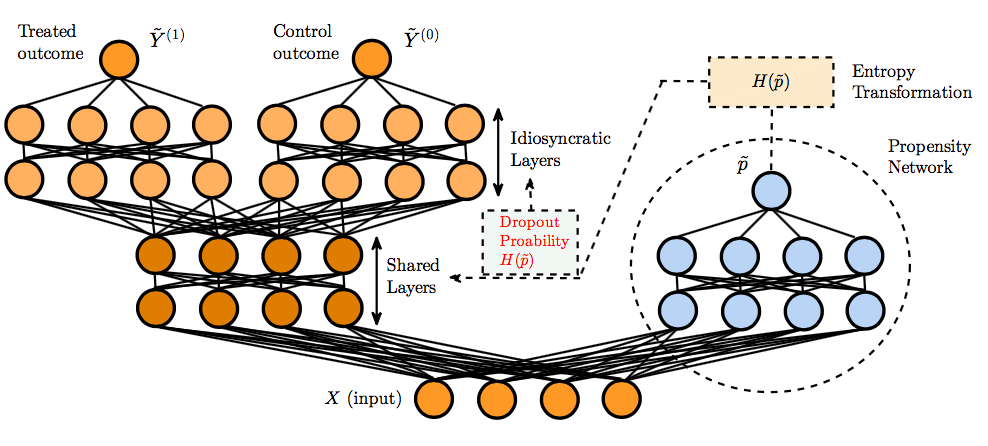
\includegraphics[width=1.0\textwidth]{figures/chapter-3/pbd-architecture.png}
	\caption{Architecture of Deep Counterfactual Networks}\label{fig:dcn-architecture}
\end{figure}

We introduce \emph{deep counterfactual networks} a novel approach to using deep neural networks for the task of counterfactual inference. Our model -- illustrated in figure \ref{fig:dcn-architecture} and described in detail in the following -- conceptualises counterfatual inference as a multi-task learning problem (see section \ref{sec:multi-task-learning}). This way, we achieve  statistical efficiency while at the same time ensuring a high degree of modelling flexibility. 

In addition, we address the  problem of the covariate shift between the factual and counterfactual dataset by utilising a novel propensity-based dropout scheme (see section \ref{sec:propensity-based-dropout}). This way, we are also able to provide confidence intervals for our predictions increasing. 

\subsection{Multi-Task Learning} \label{sec:multi-task-learning}
\emph{Deep counterfactual networks} (DPNs) make use of multi-task learning to learn a \emph{shared representation} for the potential outcomes (treated and untreated) in order to predict the individualised treatment effect $T(x)$. 

The model, illustrated in figure \ref{fig:dcn-architecture}, consists of two separate networks: A \emph{propensity-network} on the right and a \emph{potential outcomes network} on the left.
The propensity-network represents a standard feed-forward neural network consisting of $L_p$ hidden layers and $h_p^{(l)}$ hidden units for the $l^{th}$ layer. It is trained separately, and 

\subsection{Propensity-based Dropout} \label{sec:propensity-based-dropout}

\section{Training the Model}

\begin{figure}[h]
	\centering
	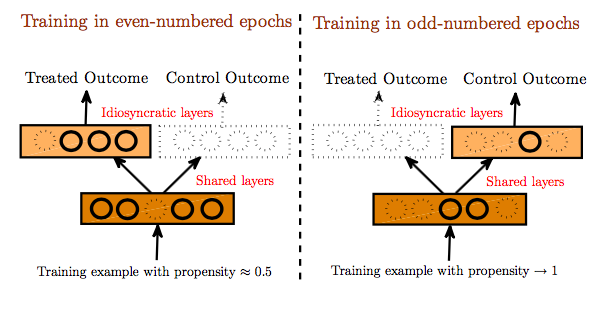
\includegraphics[width=1.0\textwidth]{figures/chapter-3/pbd-training.png}
	\caption{Visualisation of Training Algorithm}\label{fig:dcn-training}
\end{figure}
